\section{Data Collected}

The MARATHON experiment ran from January through April of 2018 in Hall A at JLab. During the experiment the HRSs were used in ``inclusive'' mode, that is each spectrometer was making an independent measurement. Throughout the discussion of the analysis each measurement by an HRS is referred to as a ``kinematic''. To switch between kinematics the LHRS was rotated around the target to different angles. The RHRS was parked at the highest angle kinematic for the entirety of the experiment since that kinematic had a very slow event rate.

\begin{table}[h]
\begin{center}
\begin{tabular}{|l|l|l|l|l|}
\hline
\textbf{Kinematic} & \textbf{E$^\prime$} (GeV/$c$) & \textbf{Angle} ($\degree$) & \textbf{Central $x$} &  \textbf{No. of Iterations} \\
\hline
\hline
0 & 3.1 & 16.9$\degree$ & 0.199 & 1 \\ \hline
1 & 3.1 & 17.577$\degree$ & 0.218 & 1 \\ \hline
2 & 3.1 & 19.115$\degree$ & 0.257 & 1 \\ \hline
3 & 3.1 & 20.578$\degree$ & 0.298 & 1 \\ \hline
4 & 3.1 & 21.93$\degree$ & 0.338 & 1 \\ \hline
5 & 3.1 & 23.213$\degree$ & 0.378 & 1 \\ \hline
7 & 3.1 & 25.594$\degree$ & 0.46 & 2 \\ \hline
9 & 3.1 & 27.778$\degree$ & 0.538 & 2 \\ \hline
11 & 3.1 & 29.917$\degree$ & 0.62 & 2 \\ \hline
13 & 3.1 & 31.732$\degree$ & 0.70 & 2 \\ \hline
15 & 3.1 & 33.562$\degree$ & 0.78 & 3 \\ \hline
16 & 2.9 & 36.12$\degree$ & 0.82 & 2 \\ \hline
\end{tabular}
\caption{This table describes the key variables that define each kinematic.}
\label{tbl:kins}
\end{center}
\end{table}

For all kinematics the LHRS momentum was set to $3.1$ GeV/$c$. The RHRS momentum was set to $2.9$ GeV/$c$ due to limitations of the dipole magnet. The kinematics are numbered based on the originally proposed kinematic settings. Due to time limitations, not every kinematic was measured. During the data taking the $x$ and $Q^2$ values of the data were studied and it was found that there was sufficient overlap between kinematics without the skipped kinematics. Plots showing this overlap can be seen in Figure \ref{fig:kin_plots}. A few kinematics were measured more than once when the run period was extended. Individual iterations of a kinematic are treated as independent measurements for the sake of analysis. Table \ref{tbl:kins} shows the variables that define each kinematic.

\begin{figure}[h]
\begin{center}
	\includegraphics[width=\textwidth]{./analysis/fig/kin_plots.png}
	\caption{These plots show the $x$, $Q^2$, and $W^2$ coverage of all of the MARATHON kinematics. Each kinematic overlaps with the previous and successive kinematic, giving complete coverage of the proposed range of the experiment.\cite{Tong}}
	\label{fig:kin_plots}
\end{center}
\end{figure}

\section{Analysis Outline}
\label{sec:analysis_outline}
This chapter will go over the analysis of the data collected in the MARATHON experiment. An outline of the analysis process is as follows:
\renewcommand{\labelenumii}{\roman{enumii}.}
\begin{enumerate}
	\item For each run:
	\begin{enumerate}
		\item Apply cuts to data
		\item Calculate the electron yield and bin data in $x$
		\item Apply livetime correction
		\item Apply target boiling correction
		\item Calculate target boiling uncertainty
		\item Calculate beam charge and add it to the kinematic charge total
	\end{enumerate}
	\item For each kinematic:
	\begin{enumerate}
		\item Sum the yields from all runs in the kinematic
		\item Apply charge normalization
		\item Sum the target boiling uncertainties and apply them to the data
		\item Drop the first and last bins as they are near the edge of the acceptance
	\end{enumerate}
	\item For production of a ratio, the kinematic yields for two targets are divide ($^3$He and $^2$H in the case of this thesis)
	\item Combine all kinematics by weighted average, weighted by uncertainty
	\item Apply remaining corrections:
	\begin{enumerate}
		\item Endcap Contamination subtraction
		\item Charge Symmetric Background subtraction
		\item Target energy loss correction
		\item Coulomb correction
		\item Radiative Corrections
		\item Bin centering correction
	\end{enumerate}
\end{enumerate}
This analysis procedure will yield the $\nicefrac{F_2^{^3\textrm{He}}}{F_2^{^2\textrm{H}}}$ structure function ratio. From there, the A=3 isoscalar EMC ratio can be extracted by applying an isoscalar correction. Also, the $\nicefrac{F_2^n}{F_2^p}$ nucleon structure function ratio can be extracted using the methodology described in Section \ref{sec:F2ratio}.

\section{Yield and Yield Ratio Calculation}

The MARATHON experiment measured yield ratios. This method allows us to cancel many systematics that would otherwise plague a full cross section analysis. By taking data for each target at the same kinematics, acceptance effects are identical. This data taking technique means that with reasonable acceptance cuts, a ratio of target yields is wholly equivalent to the ratio of cross sections.

Calculating the the yield ratios requires first calculating the yield for each target. The yields calculated are binned in Bjorken $x$. The bins are 0.03 wide. The bin centers are defined by segmenting the range of 0 to 0.99 by 0.03 (i.e. the bins are centered at 0.015, 0.045, 0.075, etc.). The yield of each bin is calculated using this simple equation:
\begin{equation}
	\text{Yield} = \frac{\text{Counts}}{\text{Scattering Centers} \cdot \text{Charge}} \cdot \text{Corrections}
	\label{eqn:yield}
\end{equation}
Here ``Counts'' are the number of electrons measured that pass the cuts placed on the data and fall into that bin, ``Scattering Centers'' are the number of nucleons in the target (calculated from the target thickness, mass, and mass number $A$), and ``Corrections'' are physics or systematic effects that are otherwise unaccounted for in the data. Dividing by the ``Charge'' in each kinematic, gives us the ``Charge-Normalized Yield'', that is the expected electron count for each unit of charge incident on the target.

As described in Section \ref{sec:analysis_outline}, the charge-normalized yield is calculated for each target on a per-kinematic basis. For each kinematic, the target ratios are then calculated. This is done simply by dividing the two yields and propagating the associated uncertainties. The equations for taking the ratio are:
\begin{align}
	\text{Ratio} = \frac{\text{Yield}\left(^3\text{He}\right)}{\text{Yield}\left(^2\text{H}\right)} \\
	\sigma_{\text{Ratio}} = \text{Ratio}\sqrt{\left(\frac{\sigma_{\text{Yield}\left(^3\text{He}\right)}}{\text{Yield}\left(^3\text{He}\right)}\right)^2 + \left(\frac{\sigma_{\text{Yield}\left(^2\text{H}\right)}}{\text{Yield}\left(^2\text{H}\right)}\right)^2}
\end{align}

Once the per-kinematic yield ratios are calculated, each kinematic has its edge bins dropped, that is the lowest and highest $x$ bin. This is because these bins are located at the edge of the acceptance of the spectrometer with low counting rates and large uncertainties. After this is done, all kinematics are combined through a weighted average. The ``weight'' is the uncertainty on the measurement in that bin. The equations for the weighted average are:
\begin{align}
	\text{Average} = \frac{\sum\limits_{i} \frac{\text{Ratio}}{\sigma^2_\text{Ratio}}}{\sum\limits_{i} \frac{1}{\sigma^2_\text{Ratio}}} \\
	\sigma_\text{Average} = \frac{1}{\sum\limits_{i} \frac{1}{\sigma^2_\text{Ratio}}}
\end{align}
Once all corrections have been applied, this calculated weighted average is the final result for the yield ratio.

This chapter will explain the cuts and corrections that go into this calculation as well as the calibrations performed to make the measurements accurate.

%\section{Calibrations}
%%\subsection{ADC Calibrations}

\subsection{Raster Calibration}
The raster is calibrated by defining a line that maps the raster current to positions at each BPM and the target. To do this, the slope and intercept of this line had to be determined. The slope corresponds to the conversion of raster current to position displacement. The intercept is then determined from the central position that the beam is displaced from. This section will be a general presentation of the techniques used to calibrate the raster. For a more in-depth discussion of how the raster was calibrated, see Appendix \ref{raster_appendix}.

For the horizontal raster, this was done by optimizing the reconstructed z-vertex on the target. When properly calibrated, there should be no correlation between the horizontal raster and the z-vertex. Linear interpolation between two ``bad'' calibrations is a simple way to determine the correct calibration slope.

The veritcal raster could be calibrated in a similar way by minimizing the correlation between the vertical raster and a known momentum phenomena (i.e. a $W^2$ peak). Unfortunately, such a feature does not exist within the kinematics of MARATHON data. The vertical calibration was determined using the carbon hole target. The hole is known to be $2mm$ diameter. By using the raster data, the hole can be fit in order to determine the vertical calibration slope.

The intercepts are determined by looking at the mean BPM position readings and projecting these to the target. This position will correspond to the mean value of the rasters as well. Using the beam position, raster current, and calibration slope the calibration intercept can easily be determined.


\section{Corrections}

When analyzing the data, there are several corrections that need to be made. These are due to various physical or systematic effects that took place during the experiment. These effects have been studied in order to determine a ``correction factor'' that can be applied to the data.

\subsection{Target Boiling}
\label{sec:boiling}

When the beam is incident on the target, it deposits heat into the gas. This causes a density fluctuation of the gas referred to as ``target boiling''. The target does not actually boil, however that is the standard nomenclature for a density fluctuation in a gas target. When the density of the target changes, it changes the effective target thickness as seen by the beam. When the target thickness changes, there is a changed number of scattering centers which will lead to a change in the number of electrons recorded. Specifically, heating will decrease the target density which will decrease the number of scattered electrons.

The density changes are a function of the current on the target. Each run is taken at a single current so that the correction can be applied run by run. The correction is approximately linear for small deviations in current. A study of the effect during beam ramping found that the density settles very quickly. This means that so long as we cut events that occur with the beam off, it is unnecessary to take into account the beam ramping when correcting for this effect.

To determine the correction, a dedicated set of runs was taken with the Left HRS spectrometer at $16.8\degree$ and 3.1 GeV. At this kinematic, several data runs were recorded with varying current between them. Each of these runs were analyzed with the standard data cuts to determine the yield. This allows for the yield to be determined as a function of beam current.

Now that the yields have been determined as a function of beam current, they can be plotted and fit. The data is fit with a quadratic polynomial. This fit is constrained to require no correction (a correction factor of 1) at zero current. This is because the density must be the nominal fill density when there is no beam heating. During analysis the average current is calculated for a run (ignoring beam trips). The average current is then used to calculate the target density correction with the fit function. The correction is then applied on a run-by-run basis by multiplying the number of scattering centers by this correction factor (or equivalently dividing the yield by the correction factor). Figure \ref{fig:boilcor} shows the correction factors for each target.\cite{boiling}

\begin{figure}
	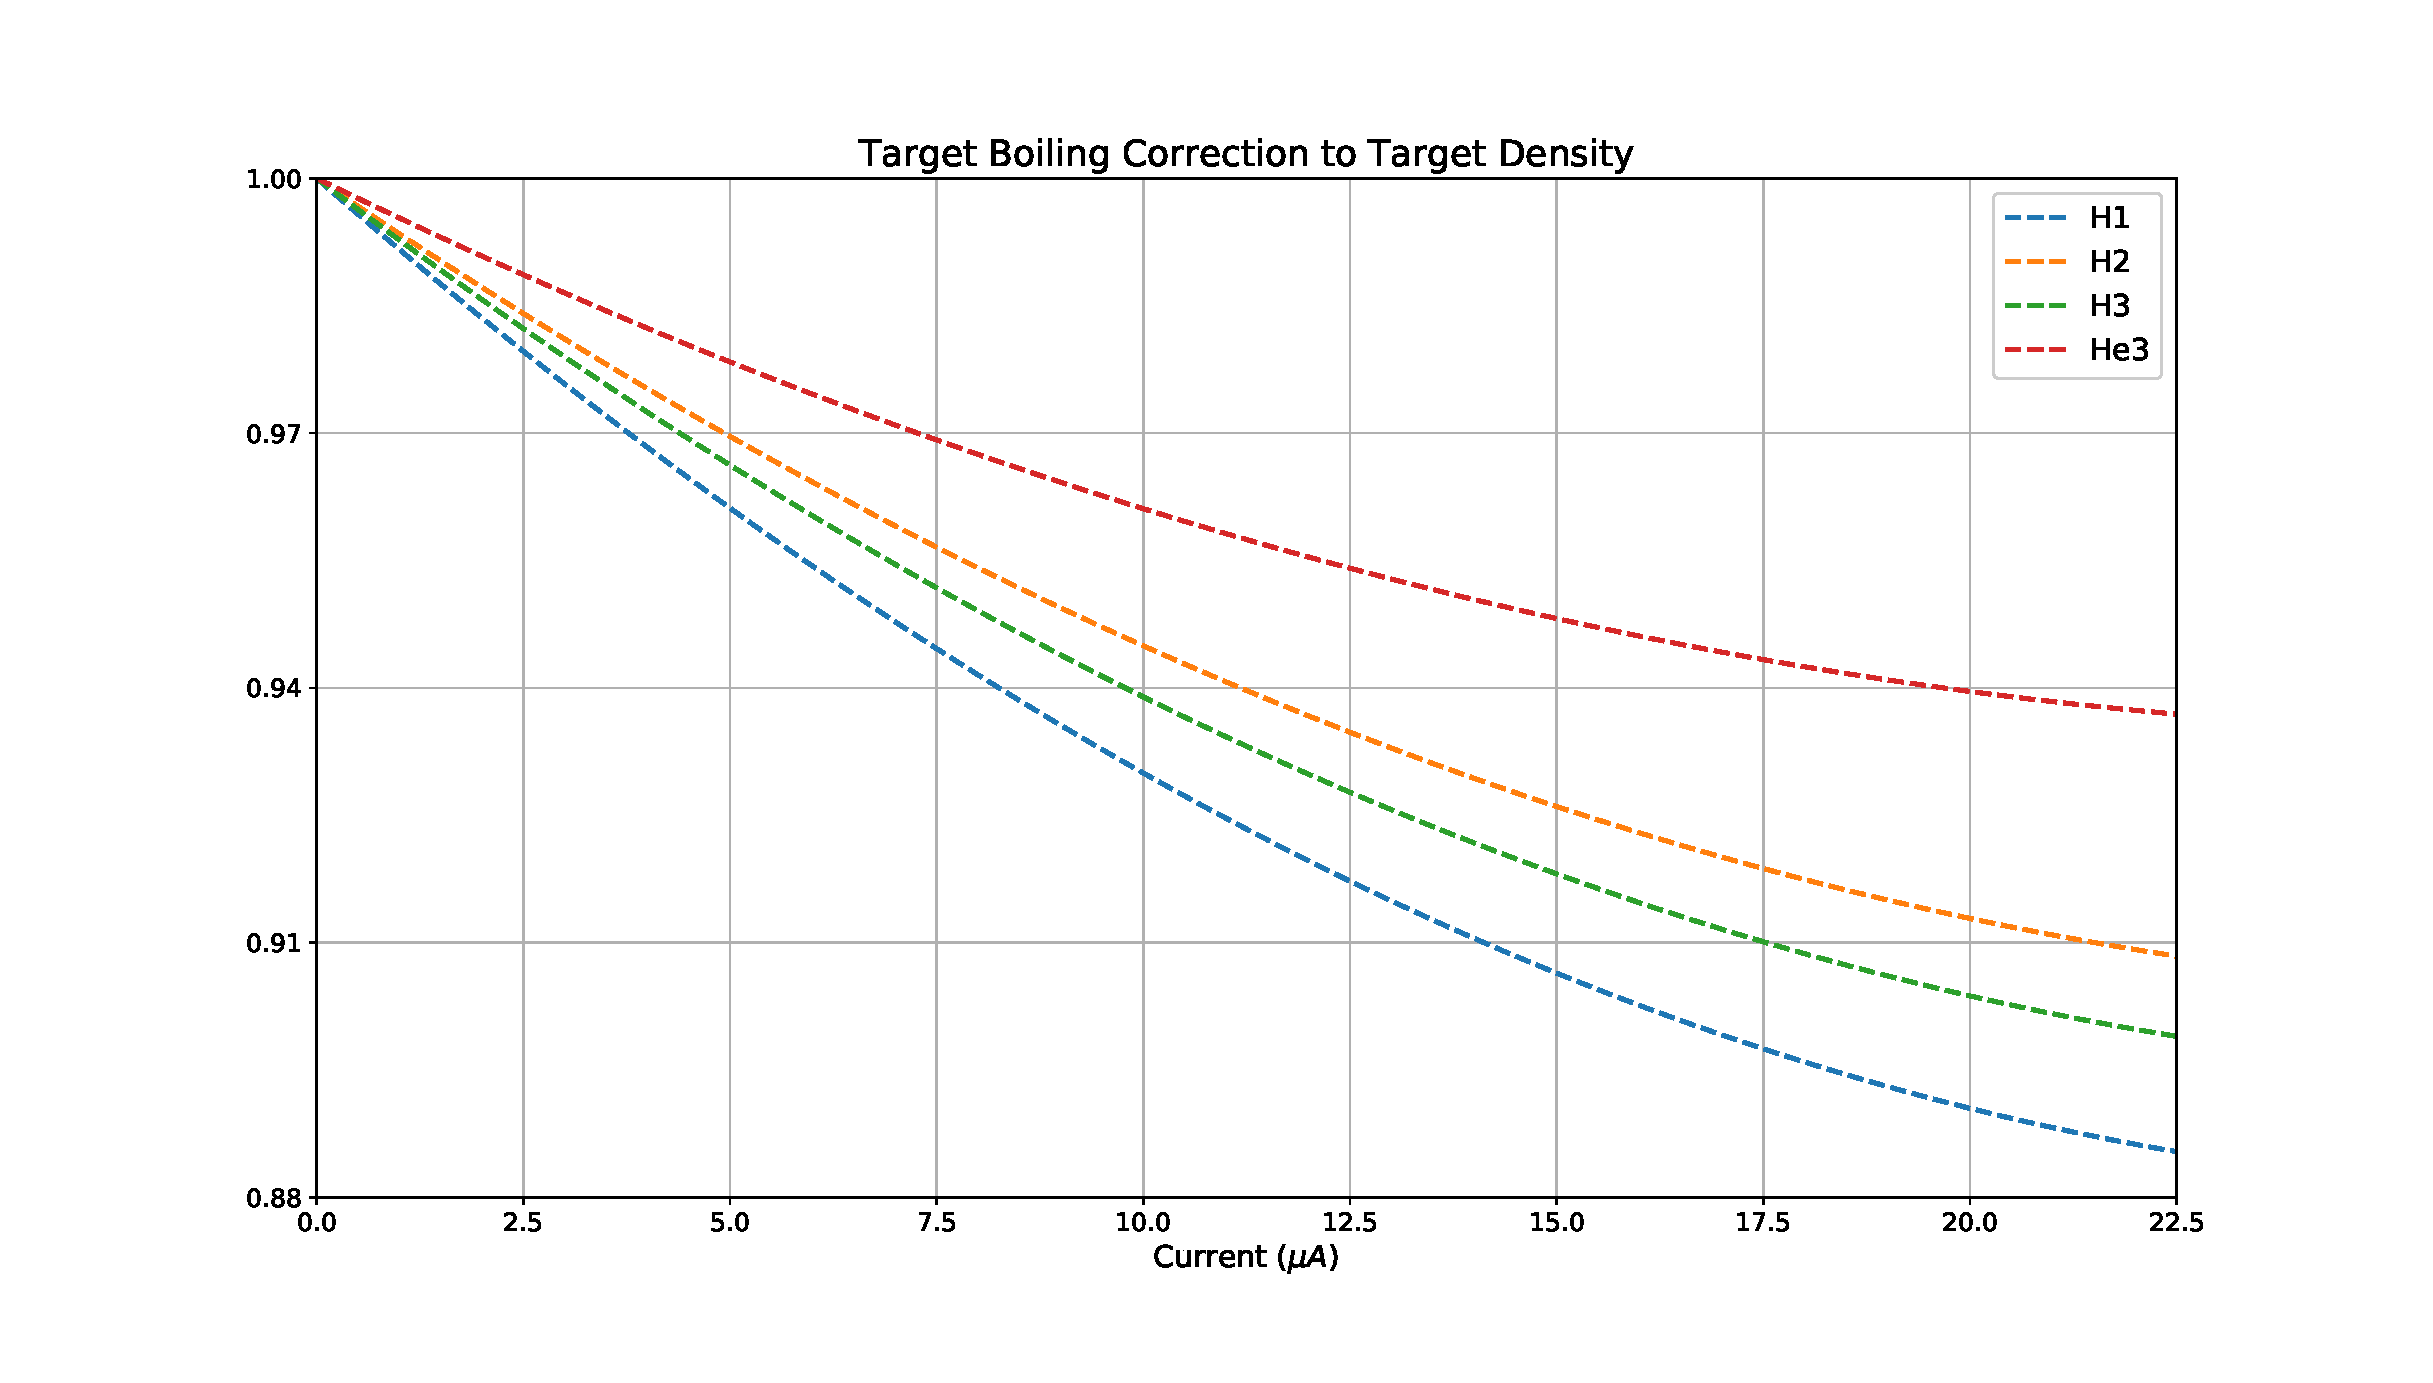
\includegraphics[width=\textwidth]{./analysis/fig/boil_cor.eps}
	\caption{Beam heating effects are manifested as a multiplicative correction to the target density}
	\label{fig:boilcor}
\end{figure}

%\begin{figure}
%	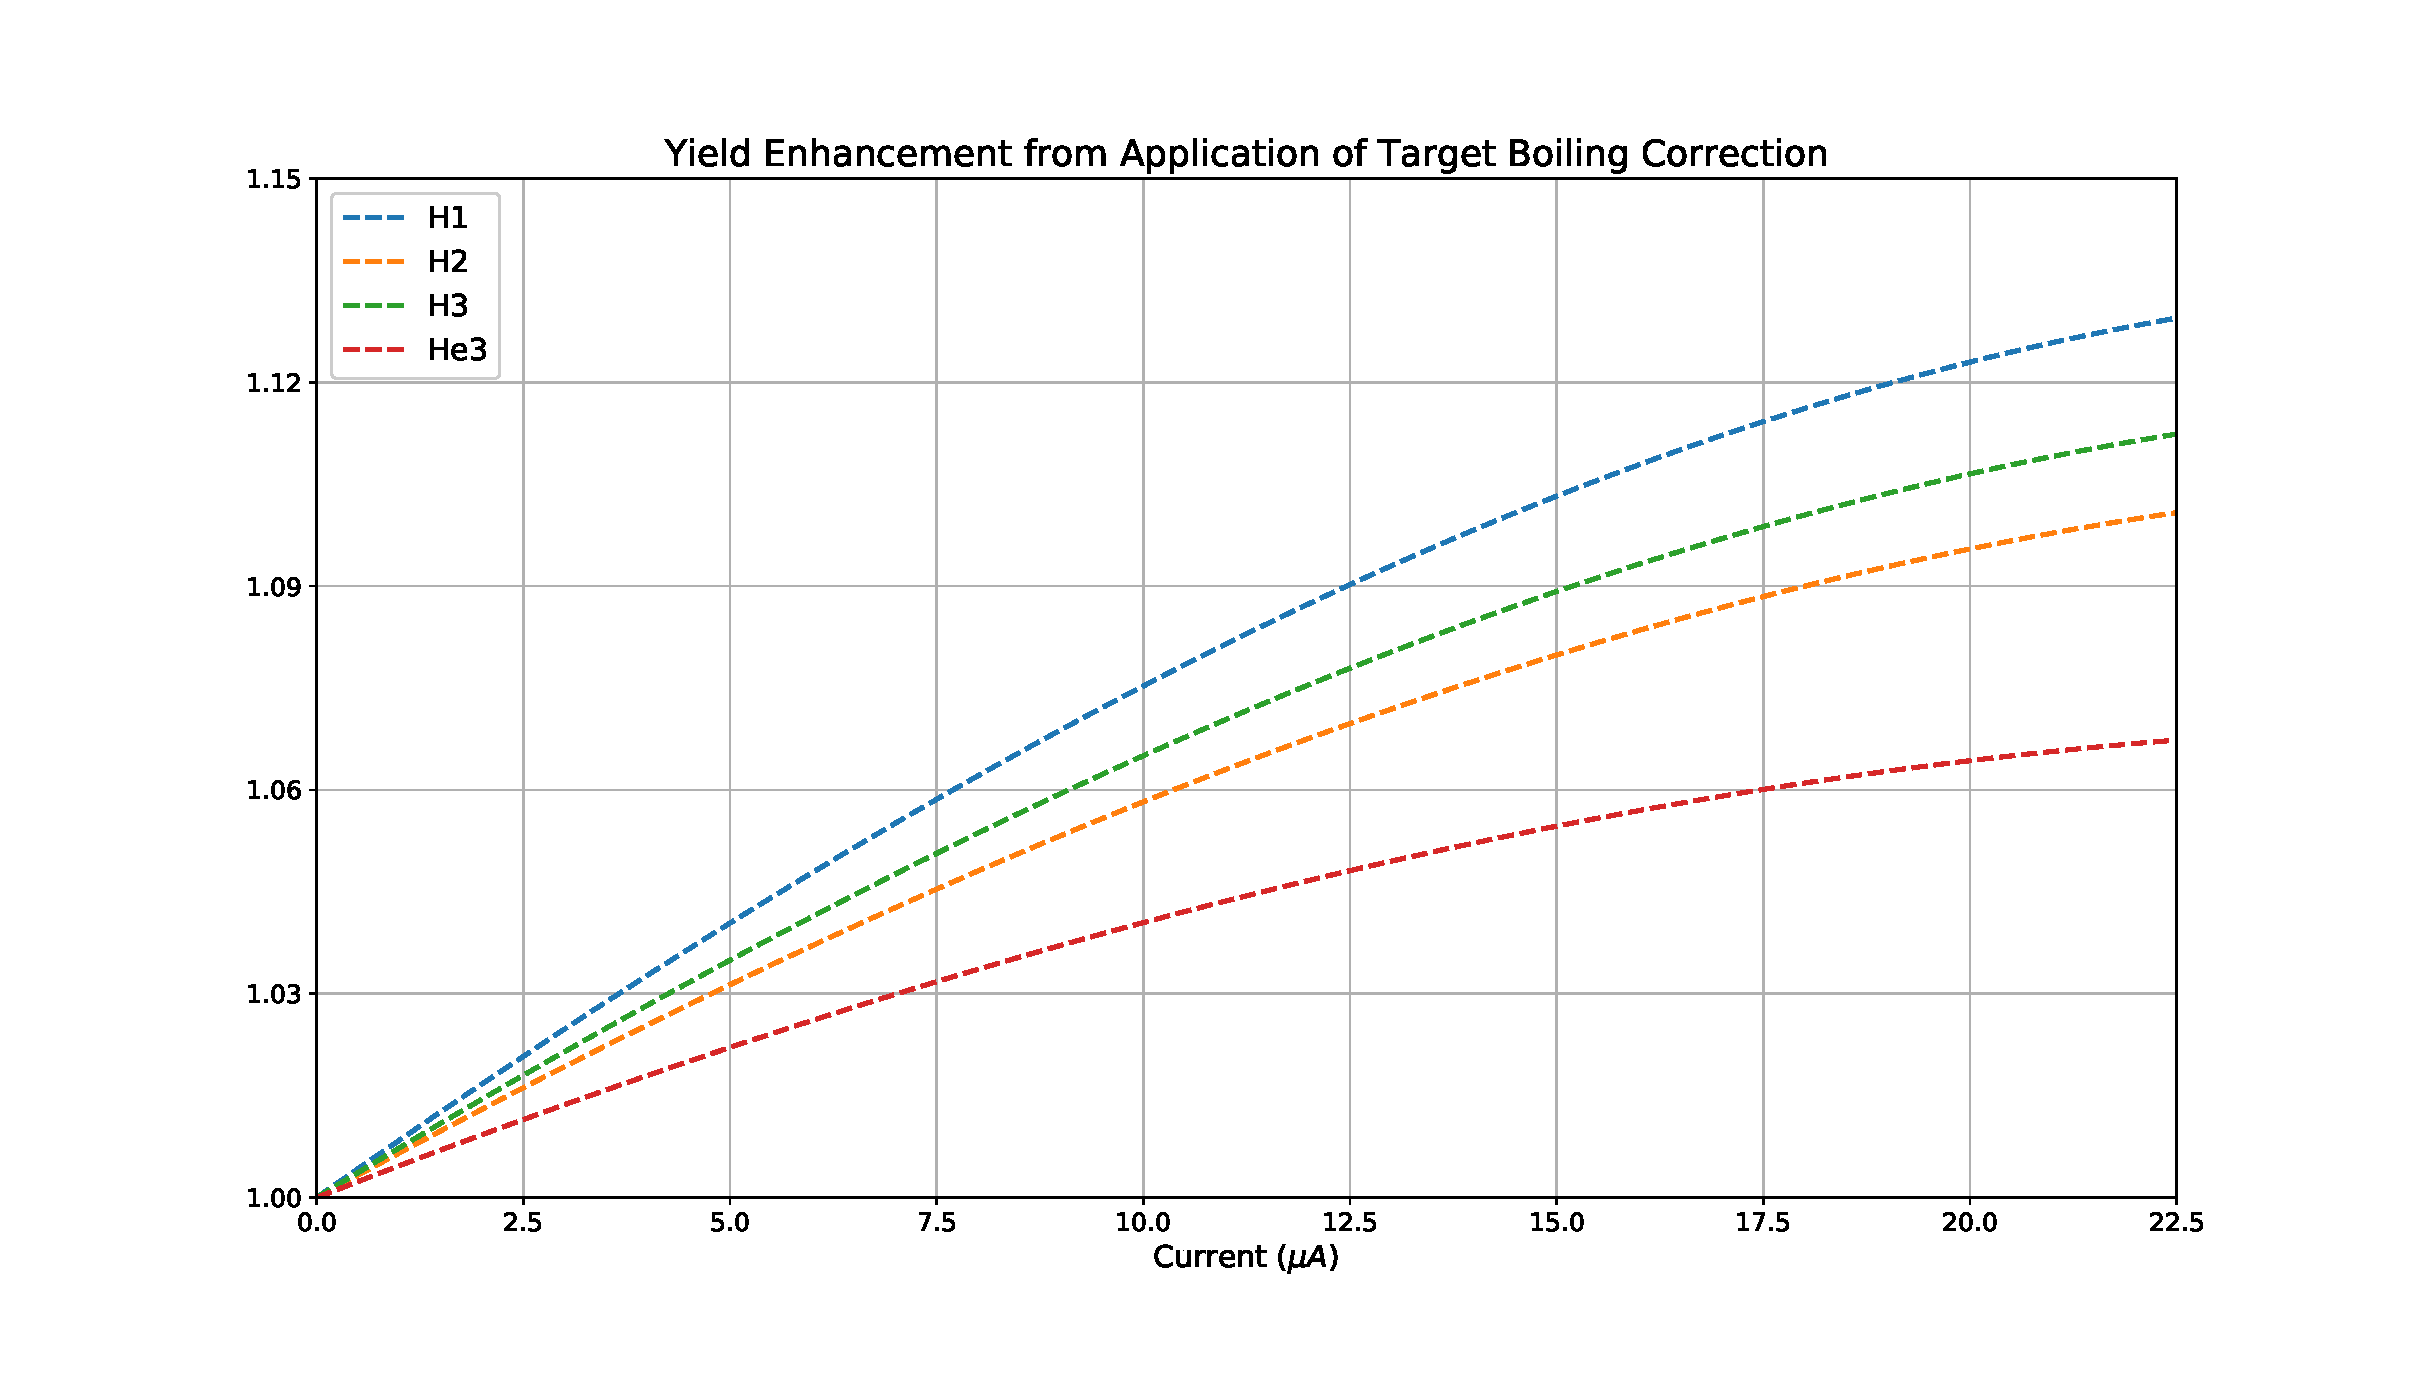
\includegraphics[width=\textwidth]{./analysis/fig/boil_yield_cor.eps}
%	\caption{Target density corrections cause a multiplicative enhancement to the yield}
%	\label{fig:boilyieldcor}
%\end{figure}

\subsection{Target Endcap Contamination}
\label{sec:ecc}

The gas targets used in this experiment are housed in aluminum cells as described in Section \ref{sec:gas_cell}. The thickness of the aluminum greatly exceeds the thickness of the gas and will contribute background that can survive the cuts placed on the data. By quantifying this contribution, the events that originate from the cell endcaps can be subtracted from the final results.

To determine this contribution, the empty cell is used. The empty cell, being an exact replica of the gas target cells with a vacuum inside, allows us to approximately isolate the contribution of the cell walls to the data. The empty cell and the target being studied are compared by calculating the yields on a kinematic-by-kinematic basis and normalizing them by charge and endcap thickness.

The normalization to the endcaps for each target must be done in two parts. This is because each endcap is not the same thickness. When calculating the yield for a target, it is assumed that any contamination upstream (downstream) of the center of the target must originate from the upstream (downstream) endcap. The two halves are then combined to arrive at the endcap thickness normalized yield. This yield calculation only has livetime corrections applied. All cuts are applied except for target length, which is adjusted to only include events upstream (downstream) of the center of the target.

The data for the target being studied and the normalized empty target are then binned in Bjorken $x$. Dividing the empty cell data by the gas target data then gives an approximation of the fractional contribution of the cell walls to the electron data. As this correction is applied to the final results, the contamination corrections for the targets are divided by each other to create the correction to the target ratios. These results are then fit with the functional form $1\pm e^{Ax+B}$. The choice of adding or subtracting the exponential is done by determining if the correction is greater or smaller than 1. The fit function and the covariance matrix of the fit are used to apply the correction to the final results as well as determine the uncertainty contribution of this correction.

\subsection{Charge Symmetric Background Subtraction}

As an inclusive scattering experiment, we are particularly susceptible to background from charge symmetric processes from the target. That is events which involved the production of both an electron and a positron, rather than the electron simply scattering. To study this, the polarity of the LHRS was reversed so that positively charge particles are directed into the detectors rather than negatively charged particles. With this setting, a number of runs were taken in kinematics 0 through 5. These runs were taken with all targets, just as the electron data was taken. This allows for a measurement of the positron yield which corresponds to a measure of the charge symmetric background.

This measurement allows us to determine the proportion of electrons that originated from pair production. Applying the same cuts and as the electron data allows us to determine the charge normalized positron yield. Unlike in the electron analysis, it was noted that there was significant pion contamination in the positron data. This pion contamination had to be subtracted in order to get an accurate calculation of the positron yield. This is achieved by fitting the main pion peak and the subtracting the tail of the fit which survives the cuts applied from the positron data.

The charge normalized positron yields over these kinematics are then combined (using the same methods as the electron yield) and binned in Bjorken $x$. This was then divided by the charge normalized electron yield. This is a fractional measure of the charge normalized background contamination. The ratio is then fit with an exponential of the form $e^{Ax + B}$, where $A$ and $B$ are the fit parameters. These fits are shown in in Figure \ref{fig:positrons}.

This correction is applied to the final yield ratio results. Both the numerator and denominator must have the charge symmetric background subtracted. Each target yield in the ratio is scaled by $1 - \left(\textrm{Charge Symmetric Background Fit}\right)$. For each bin, the fit is calculated at the bin center.

\begin{figure}
	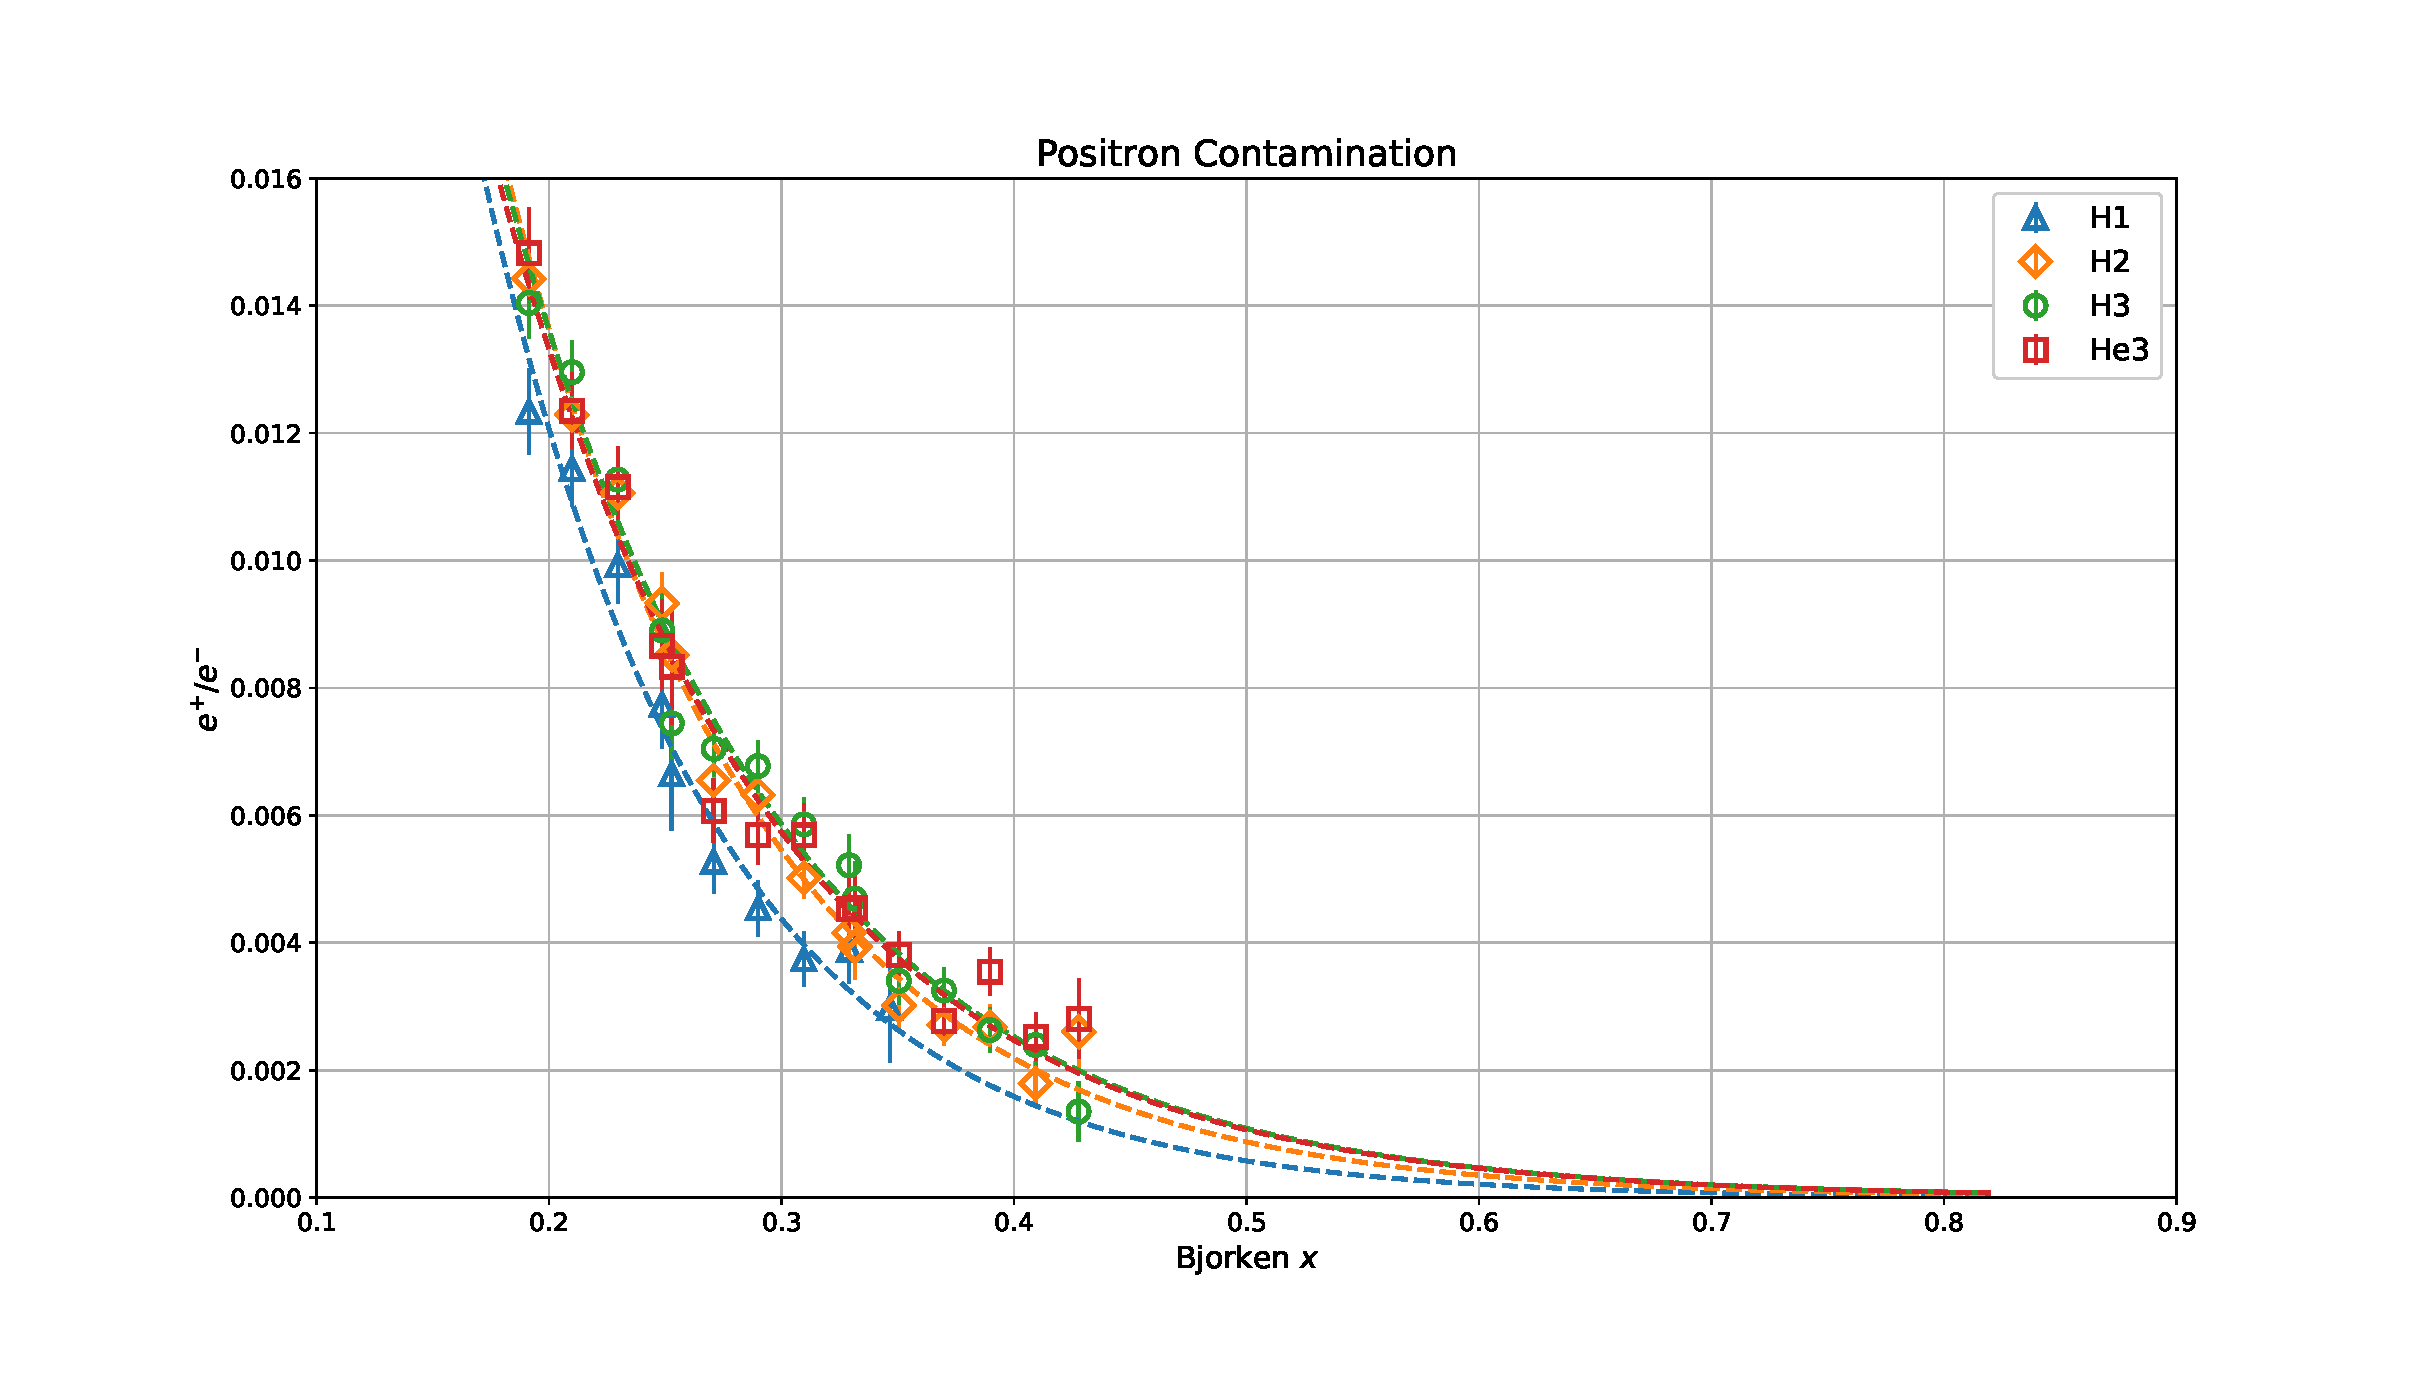
\includegraphics[width=\textwidth]{./analysis/fig/positrons.eps}
	\caption{Charge symmetric background correction}
	\label{fig:positrons}
\end{figure}

\subsection{Computer Deadtime Correction}

Our DAQ unable to continuously record data. While we can probabilistically determine the mean time spacing between events, in the real world events can deviate greatly from these means. Sometimes events will occur that are too close in time for our DAQ to record as the computer has not completed recording the previous event. Deadtime is a function of event rate; when events happen more rapidly, there is a higher chance that events will occur too closely in time to be recorded.

When deadtime is low and the number of recorded events is high, it is a reasonable assumption that the events recorded will accurately reflect the distribution of events in the ``zero-deadtime limit''. In this case correcting for the deadtime is simply done by scaling the number of events by the ``livetime'' of the experiment.

The computer livetime was measured using the Trigger Supervisor and scalers in each HRS. The trigger signals generated from detector signals are copied and sent to both the Trigger Supervisor and a scaler unit. The Trigger Supervisor is subject to the computer deadtime event loss discussed here. The scaler unit, on the other hand, simply increments a register when a trigger signal is received. The ratio of these the number of events recorded by these two systems gives a measure of the livetime of the measurement. The livetime is defined on a run-by-run basis as:

\begin{equation}
DT = \frac{\Sigma \mathrm{Triggers_{TS}}}{\Sigma \mathrm{Triggers_{Scaler}}}
\end{equation}

In an ideal world, the deadtime will be identical for all runs within a kinematic. However, the deadtime is measured on a run-by-run basis and is applied as such in order to account for any deviations from this assumption. The average deadtime for each target in each kinematic is plotted in Figure \ref{fig:deadtime}.

\begin{figure}
	\includegraphics[width=\textwidth]{./analysis/fig/deadtime.eps}
	\caption{Deadtime per kinematic}
	\label{fig:deadtime}
\end{figure}

\subsection{Radiative Corrections}

The Deep Inelastic Cross Sections being studied are the Born approximation of a single-photon exchange. The measurement however, contains contributions from higher order processes that will increase the measured cross section. Using a model, the contributions can be corrected for and removed from the measurement.

The experiment used a software package called $\texttt{T2\_EXTERNALS}$ that calculates both the Born cross section and the radiated cross section for a given target at a kinematic set $(E,E^{\prime} ,\theta )$.

\subsection{Isoscalar Corrections}

\subsection{Bin Centering Corrections}

The cross-section over the width of a bin is not constant. This means that the measurement does not correspond with the true cross section at the center of the bin. Using a model that matches the shape of our data well, the location of the measurement within the bin can be calculated. This is done by calculating the expectation value of the model within that bin and determining the $x$ value corresponding to this value. The expectation value is given by
\begin{equation}
	\langle f_{\rm measured}\rangle = \frac{1}{\Delta x}\int_{x_{\rm low}}^{x_{\rm high}} f\left( x \right) dx,
\end{equation}
where $f$ is a function representing the chosen model. In practice, the $x$ value does not need to be calculated if the data will be reported at the bin center. Rather, the correction is simply the ratio of the model at the bin center. This is written as
\begin{equation}
	\sigma_{\textrm{Bin Centered}} = \frac{f\left(x_{\textrm{Bin Center}}\right)}{\langle f_{\rm measured}\rangle} \sigma_{\rm measured}.
\end{equation}

This correction must be applied to both targets in the ratios. That is, the ratio must be multiplied by the correction to the numerator and divided by the correction to the denominator.\cite{wtsydp}

\subsection{Coulomb Corrections}

Corrections must be made for the effect of the charge of the target on the scattered electron. This interaction causes the $Q^2$ of the event to shift to an effective $Q^2$ value, $Q^2_{\rm eff}$. This conversion is done with the equation
\begin{equation}
	Q^2_{\rm eff} = Q^2 \left(1 + \frac{3Z\alpha\hbar c}{2RE}\right)^{2}.
\end{equation}
In this equation $R$ is the hard-sphere equivalent radius of the nucleus which is defined as $R=\left[\left(\nicefrac{5}{3}\right) \langle r^{2}\rangle\right]^{\nicefrac{1}{2}}$ where $\langle r^2\rangle$ is the root-mean-squared radius of the nucleus.\cite{coulomb}

Using $x=\frac{Q^2}{2M\nu}$, it is clear that a shift in $Q^2$ will result in a proportional shift in $x$. Using a model cross-section, the cross section is calculated at both the nominal $x$ and at $x_{\rm eff}$. As the results have been bin centered, this calculation uses a nominal $x$ at the center of the bin. This will lead to the correction
\begin{equation}
	\sigma_{\textrm{Coulomb Corrected}} = \sigma_{\rm data} \frac{\sigma_{\rm model}\left(x_{\rm eff}\right)}{\sigma_{\rm model}\left(x\right)}.
\end{equation}

This correction must be applied to both targets in the ratios that are calculated.

\section{Cuts}
When analyzing the data, cuts must be applied to give a set of ``good electrons''. Cuts are a defined set of conditions that must be met by an event to be classified as ``good''. In this analysis, the cuts can be classified in two categories: Particle Identification and Acceptance. Particle Identification cuts are used to ensure that all events being studied are electrons. Acceptance cuts are used to ensure that all events passed through areas of the spectrometer that are well constrained by the spectrometer optics.

\subsection{Particle Identification}

Particle Identification (PID) cuts are applied to the detectors in the HRSs. The first PID cut is referred to as the ``Trigger 2'' cut. This cut requires that an event fires Trigger 2 (Trigger 5 for the RHRS) which is the (S0 \&\& S2) \&\& Cherenkov trigger. This cut requires that S0 and S2 fire, which will ensure proper event timing and tracking. Ensuring that the Cherenkov fires is the first step to limiting the events to electrons. As described in Section \ref{sec:cer}, the Cherenkov will, in most cases, only fire for electrons due to the 4.8 GeV/\textit{c} momentum threshold for pion detection.

The next cut is the ``1-Track'' cut. This cut requires that an event must have only one track through the spectrometer associated with it. A single track assures that the event corresponds to a single electron. When multiple tracks are present, there is a risk that tracking and spectrometer readings will be incorrect.

There is a cut placed on the $W^2$ of an event. The goal of MARATHON is to measure the DIS cross section ratios. A cut on $W^2$ must be placed in order to ensure that all events are from the DIS region and to reject events that originate from Resonance scattering. This cut is placed for $W^2>3$  GeV$^2$/\textit{c}$^4$.

A cut is placed on the Cherenkov signal. This cut is placed on the ADC spectrum of the Cherenkov. For the LHRS the cut is at 1500; the cut is placed at 2000 for the RHRS. While the Cherenkov will generally only fire for electrons, there are a small number of high momentum pions that are capable of creating a signal. The high momentum threshold for pions means that any pions that do create a signal will create a very small signal. This can be seen in Figure \textbf{blah}. By placing this cut, the pion peak is completely removed while the electron peak is nearly completely allowed to pass.

The final PID cut is on the ratio of the energy of the particle to the momentum of the track ($E/p$). For electrons, which have a low mass compared to the energy scale of the experiment, the $E/p$ is expected to be approximately 1. Any particle of larger mass that passes the ``Trigger 2'' cut (and thus created a Cherenkov signal) will have an $E/p$ value significantly smaller than 1. In order to eliminate these non-electron events a cut on $E/p$ is placed at $0.7$ for both arms. This spectrum can be seen in Figure \textbf{blah}.

\subsection{Acceptance}

Acceptance cuts are placed on the kinematic region that the spectrometer is sensitive to. These cuts are applied to the tracking variables ``Target $\phi$'', ``Target $\theta$'', and ``$\delta p$''. Target $\phi$ is a measure of the rotation in the plane of the hall floor. The value is the angular displacement from the central angle of the spectrometer. Target $\theta$ is the vertical angular displacement of the scattered electron. $\delta p$ is the deviation of the momentum of the scattered electron from the central momentum of the spectrometer. The RHRS also has a cut placed on the focal plane. These cuts are defined by looking at the acceptance of the spectrometer. Examining the acceptance of each spectrometer, cuts were placed around the area where the events were concentrated. The areas where events ``fell off'' were considered to be outside of the acceptance of the spectrometer. This is also how the focal plane cuts were determined for the RHRS.

The other acceptance cut that is applied is to the target length. This cut is applied to the ``z-Target'' value of an event, where the event happened in the target along the axis of the beamline. This cut is used in order to minimize the amount of Endcap Contamination events that need to be corrected for. The cut is defined on a kinematic-by-kinematic basis, with higher kinematics having more of the target length allowed to pass the cut due to a smaller endcap contribution to the overall event rate. These cuts are defined in Table \ref{tbl:ztar}.

\begin{table}
\begin{center}
\begin{tabular}{|c|c|}
\hline
\textbf{Kinematics} & \textbf{z-Target Acceptance (m)}\\
\hline\hline
0 - 4 & $-0.08$ - $0.1$ \\ \hline
5 - 7 & $-0.09$ - $0.1$ \\ \hline
9 - 11 & $-0.095$ - $0.1$ \\ \hline
13 - 15 & $-0.1$ - $0.105$ \\ \hline
16 & $-0.105$ - $0.11$ \\ \hline
\end{tabular}
\caption{This table shows the range of the target, along the beam axis, that events are accepted from. This is done to minimize contamination from the endcaps of the targets.}
\label{tbl:ztar}
\end{center}
\end{table}
